\chapter{ILLUSTRATING RESTful WEB}
\begin{spacing}{1.5}
Web APIs and RESTful Web services are hypermedia applications consisting of interlinked resources, oriented towards machine consumption. The orientation towards machine consumption manifests mainly in that the interactions between RESTful services and their clients are generally done with structured data (e.g. XML, JSON), as opposed to the standard Web document markup language, HTML, which is a human-oriented presentation language. In their structure and behavior, RESTful Web services are very much like common Web sites. 

Figure: \ref{fig:hotel_booking} illustrates an example RESTful hotel booking service, with its resources and the links among them. The “service description” is a resource with a stable address and information about the other resources that make up the service. It serves as the initial entry point for client interaction. 

\begin{figure}
        \centering
        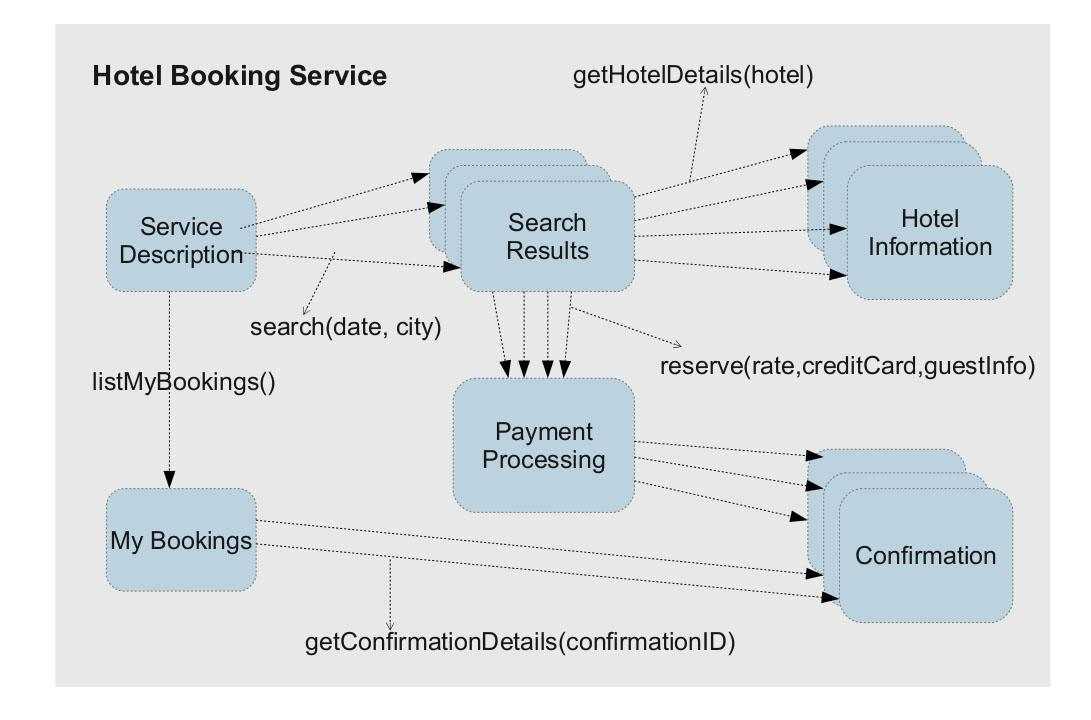
\includegraphics[scale=0.4]{images/hotel_booking.jpg}
        \caption{Structure of an Example Service}
        \label{fig:hotel_booking}
\end{figure}
The service description resource contains a form for searching for available hotels, given the number of guests, the start and end dates and the location. The search form serves as a link to search results resources, one per every unique combination of the input data — the form prescribes how to create a URI that contains the input data; the URI then identifies a resource with the search results. As there is a large number of possible search queries, there is also a large number of results resources, and the client does not need to know that all these resources are likely handled by a single program on the server. 

The search results are modeled as separate resources (as opposed to, for instance, a single data-handling resource that takes the inputs in an input message), because it simplifies the reuse of the hotel search functionality in other services or in mashups (lightweight compositions of Web applications), and it also enables caching of the results. With individual search results resources, creating the appropriate URI and retrieving the results (with HTTP GET) is easier in most programming frameworks than POSTing the input data in a structured data format to one Web resource, which would then reply with the search results. 
            
The service description also contains a link to a page with the bookings of the current user (which requires authentication functionality). With such a resource available to them, client applications no longer need to store the information about performed bookings locally.

Search results are a list of concrete rates available at the hotels in the given location, for the given dates and the number of guests. Each item of the list contains a link to further information about the hotel (e.g. the precise location, star rating and other descriptions), and a form for booking the rate, which takes as input the payment details (e.g. credit card information) and an identification of the guest who is going to stay in the room. The booking data is submitted (POSTed) to a payment resource, which processes the booking and redirects the client to a confirmation resource. The content of the confirmation can serve as a receipt.
             
Finally, the “my bookings” resource links to the confirmations of the bookings done by the authenticated user. The confirmations may further provide a way of canceling the reservation (not shown in the picture). 
           
Together, all these resources form the hotel booking service. However, the involved Web technologies actually work on the level of resources, so service is a virtual term here and the figure shows the service in a dashed box. 
        
So far, the description of the example hotel reservation service has focused on the hypermedia aspect: we described the resources and how they link to each other. Alternatively, and in fact more commonly, we can also view the service as a set of operations available to the clients — as an API. The search form in the homepage represents a search operation, the hotel information pages linked from the search results can be viewed as an operation for retrieving hotel details, the reservation form for any particular available rate becomes a reservation operation, and so on. 
          
While the resources of a service (the nouns) form the hypermedia graph (shown in Fig. 3.1), a programmer making a mashup or an automated client program rather thinks of the operations that can be invoked; therefore public RESTful Web services are generally called APIs and are described in terms of the operations. The following might be a typical operation description: 

The operation \texttt{getHotelDetails()} is invoked using the method GET at \\
\texttt{http://example.com/h/\{id\}}, with the ID of the particular hotel replacing the parameter id. It returns the hotel details in an ex:hotelInformation document.
\end{spacing}